\section*{Пьеса}
\subsection*{Описание алгоритма написания книги}
\subsubsection*{\sout{Треш, угар и содомия}} % зачёркнуто
\begin{epigraph}
    --- В нас начал пропадать дух олдфагости...\\
    --- Мы перестали писать в окна любимым женщинам...
    \flushright{\normalfont Вырвано из контекста разговора об ICQ, 14 октября 2016}
\end{epigraph}

Основана на реальных событиях с минимальным вкраплением художественного вымысла.\\ 

\begin{figure}[ht!]
    \centering
    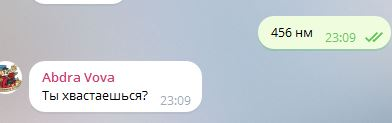
\includegraphics[width=\textwidth]{reservoirdogs}
    \caption{Славным ублюдкам посвящается...}
\end{figure}

\begin{center}
\large Действие первое и единственное % ибо уникальное
\end{center}


{\small\textttt{Пятница. Вечер. Октябрь. 14 число. 2016 год.}}


{\small\textttt{Морось. Пожалуй это лучшее слово для описания погоды, которая шаталась по улице в ту ночь, постукивая горошинами капель в окна мирно дремавших горожан. 4 представительных джентельмена, сидя за круглым деревянным столом, режутся в преферанс и перекидываются мыслишками.}}



[Vova, обращаясь к вошедшей в комнату Виктории, которую позвал Лёха]
оО, какие люди!


[Vova]
Алекс, ты уверен, что у Вика достаточно устойчивая психика для этого круговорота безумия?


[Вика зловеще хихикает]


[Vova]
Хотя нет, мы же плоды её воображения, и она сама это подстроила.


[Вика (видимо о чём то своём нам неведомом)]
Какое ехидное единоборство!


[Лёха]
Вольдемар, скоро узнаем...


[Лёха]
Антуан, я давеча нашёл прелюбопытнейшую картинку для нашей книги. \href{http://cs8.pikabu.ru/post_img/2016/10/14/5/1476431396146890414.jpg}{Не желаете взглянуть?}


[Anthony]
Пытаюсь как-нибудь привязать шутку про Билли Милигана к этой картинки: "И тут я осмотрел все свои личности" (что то в этом духе - надо додумать)


[Лёха]
Что-то типа: "Я сижу один, а меня окружают одни дураки"?


[Anthony]
Можно и сторону одиночной камеры заключения обыграть.


[Лёха]
Написание хорошего чёрного юмора — сложная задача.


[Anthony]
Вообще качественной более-менее приличной шутки.


[Лёха]
Ну в чёрном нужно ещё суметь не оскорбить всяких идиотов.


[Лёха, загадочно улыбаясь]
Или наоборот...


[Илья, улыбаясь ещё более загадочно]
Тут скорее наоборот.


[Anthony]
Точнее оскорбить так, чтобы они этого не поняли.


[Илья]
"Множественные дураки Билли Миллигана"?
"Документальный роман Дэниела Киза"


[Лёха]
"Я и мои дураки". Автобиография Билли Милигана


[Илья]
Дартаньян и три дурака


[Лёха]
Хорошо, что дураки, а не ...


[Илья смеётся]


[Anthony комментирует вышесказанное]
Оправдательная речь директора автоваза
"Хорошо, что дураки, а не ..."


[Лёха]
А не брак (здесь должна быть отсылка к переписке в вк) % вставить ссылку на соответствующую главу в книге


[Anthony]
Предлагаешь её сюда завернуть?


[Лёха]
Да.


[Anthony достаёт из рукава жестом волшебника какую то мятую бумажку сомнительной свежести и начинает читать]
У меня такой вопрос: почему слово брак означает свадьбу и негодную деталь?

Anton 10:06 pm

    Может его стоит отнести к разряду нецензурных? Т.к. только мат люди используют и для радости , и для описания печали)

Alexey 10:07 pm

    Придётся тогда писать бр*к
    И все сразу — что это за слово???!

Anton 10:07 pm

    бра*
    б*ак

Alexey 10:07 pm

    б**к

Anton 10:08 pm

    быык)

Alexey 10:08 pm

    беек

Anton 10:08 pm

    блик

Alexey 10:08 pm

    блок

Anton 10:09 pm

    баюк
    (котёнок Баюна)

Alexey 10:09 pm

    и самое неочевидное

    б-звезда-звезда-к

Anton 10:10 pm

    одним словом: хорошую вещб браком не назовут)
    так говорят они
    в смысле, пословицы
    хотя и люди тоже подойдут
    2-х смысленно
    Forwarded Messages
    Anton 13.10.16
        хотя и люди тоже подойдут

Alexey 10:12 pm

    брак всему голова
    семь раз отмерь, один раз брак

Anton 10:12 pm

    сделал брак, иди переделывай

Anton 10:13 pm

    не откладывай на завтра то, что можешь сделать браком сегодня

Alexey 10:13 pm

    брак на брак не приходится

Anton 10:14 pm

    Всемогущ бог, да хитёр брак

Alexey 10:15 pm

    Сколько человека не корми, всё равно на брак смотрит

Anton 10:15 pm

    работа не брак, сама себя не сделает

Alexey 10:16 pm

    брак браком вышибают

Anton 10:17 pm

    без труда не сделаешь брака ни черта

Alexey 10:18 pm

    нет так страшен брак, как его малюют

Anton 10:19 pm

    новая подподрубрика?
    бракованные идеи

Alexey 10:19 pm

    поговорки на новый лад?

Anton 10:19 pm

    на новый брак

Alexey 10:19 pm

    точно!

Anton 10:22 pm

    сейчас смотрю на нашу переписку и окончательно сформулировал и без того витавшую в воздухе гипотезу
    всё начинается от простейшего и эволюционирует к тому, что мы в конце будем называть идеалом - нет такого, что вдруг - бац - и нате! готово совершенство
    закон Вселенной
    шах и мат

Alexey 10:23 pm

    шах, мат и нате

Anton 10:24 pm

    НАТЕ - для двупрочтения)

Alexey 10:24 pm

    здесь в любом смысле хорошо звучит


[Илья]
не говори брак, пока не поломаешь
не всё коту качество, будет и брак
брак с возу — конвейеру легче
в ногах брака нет
глядит в книгу, видит брак


[Anthony]
брак с ленты — конвейеру легче - что-то вроде осовременивания пословиц


[Anthony]
в ногах [Болта] брака нет


[Лёха]
Они же на новый лад/брак.


[Anthony, улыбаясь]
Ну да. Ну да.


[Лёха]
Спонсор следующего текста http://www.mista.ru/pogovorki.htm

Без брака бракованные.
Брак в помощь.
Брак создал, брак и забрал.
Брак всё стерпит.
Была у собаки хата, брак пришел — она сгорела.
В ногах брака нет.
Там хорошо, где брака нет.
Вот где брак зарыт.
Вывести брак на чистую воду.
Где браки зимуют.
Брак - не тётка.
Два сапога - пара, а три - брак.
Дело пахнет браком.
Брак познаётся в беде.
Брака не хватает.
И швец, и жнец и бракоделец.


[Anthony]
А указывать ссылки как спонсоров --- интересная задумка.


[Anthony, после секундных раздумий, продолжает]
Надо будет её в книжку привить...


[Лёха]
Добрый доктор Антон сделает прививку и вашей книге.


[Илья]
Книжный грипп?


[Лёха \href{http://i5.imageban.ru/out/2014/09/04/442aff271469c9b3f514584819fcc35c.jpg}{изображает лицом доктора Хауса}]
Возможно, а может быть и книжчанка.


[Илья]
dr. Book-us


[Илья]
Хм, "Во все книжные"


[Илья]
Теория большой книги.


[Лёха]
11 литературных друзей.


[Илья шёпотом]
книжки, кофе


[Илья громче]
2 стола?


[Лёха]
шкафа, бобра, кота...


[Илья показывает большой палец вверх]
Книжки, кофе, 2 кота!


[Vova возвращаясь в комнату с кружкой свежеразлитого бренди]
Брак без водки — деньги на ветер!


[Vova, выпивая залпом весь напиток, продолжает, слегка морщась]
Семь раз отмерь, один раз брак.\\
Брак браку брак уже было?


[Anthony]
Так можно всё что угодно переделать: Было у отца 3 сына. Старший был умён, средний силён, а ещё один - бракован.


[Vova]\\
Было у отца три сына:\\
Старший умный был детина,\\
Средний был и так, и сяк,\\
Младший — откровенный брак!


[Vova, блаженно улыбаясь]
Это просто милота.


[Anthony]
Да уж пятница определённо вышла плодотворной на идеи --- попрежнему жду ваших иллюстраций с завтрашней философии.


[Лёха (уклончиво)]
Всё зависит от музы...


[Anthony]
От скучности лекции.


[Vova, хитро прищурившись]
Антон, ты опять во времени запутался — завтра ждать надо, а не по-прежнему.


[Vova]
Future Simple вместо Present Continiuos надо.


[Anthony]
Хочется ответить цитатой современного мёртвого/живого поэта/рэпера (шрёдингера?) --- сегодня завтра станет вчера.


[Vova]
С каких пор мэр Киева — репер?


[Anthony]
Это гуф - забыл Лену?


[Vova ехидно улыбается]
Я такие вещи не слушаю.


[Илья]
Кличко = Лена?


[Лёха (не совсем ясно о ком/чём?)]
Мёртвая вещь.


[Anthony]
Очень нерекомендую) особенно перед завтраком.


[Лёха]
Чтобы завтра не стало сегодня!\\
Ну или не только завтра.


[Vova]
— Не слушайте перед завтраком русский рэп.\\
— Так, помилуйте, другого-то низкосортного говна и нет!\\
— Вот никакое и не слушайте!


[Anthony]
Мне кажется или стикеры --- это какая то нездоровая тема?


[Vova изображает Фрейда]


[Лёха]
Ну не на столько же!


[Anthony]
Вывод вечера --- беседа переходит в угар, когда в ход идут стикеры.


[Лёха]
Вывод: не нужно нюхать стикеры!


[Anthony]
у нас была беседа в телеграмме. несколько идей и стикеры, но мы боялись их трогать...


[Лёха]
и куча различных смайлов всех цветов и расцветок


[Anthony]
а ещё кто-то постоянно пересылал сообщения из вк


[Anthony]
самокритичный ублюдок)


[Vova]
У меня алиби.


[Лёха]
А я в домике.


[Vova]
"самокритичный ублюдок)"



[Лёха]
юзай картинки


[Vova]
долго, дорого, нахуz не нужно.


[Vova]
Предлагаю разместить эту цитату в коментариях в коде нашего форума.


[Вика врывается в комнату и всплёскивает руками]
Вова матом ругается!


[Лёха тоном меланхоличного флегматика]
Может быть ещё ASCII артов и в каждой странице?


[Vova]
Вова так разговаривал каждым летом, когда во дворе бегал)


[Очередной ох-вдох от Вики]


[Vova, подмигивая]
Это красный, детка!


[Anthony тоном диванного эксперта]
Вова не ругается, а ясно формулирует свои эмоции в словестных выражениях определённой направленности;


[Anthony полушёпотом добавляет]
направленность снова 2смысленна.


[ТОном учителя младших классов Виктория]
Определенной нравственности*


[Anthony]
К чёрту нравственность --- Только водоворот безумия --- только bookcore!
